% Options for packages loaded elsewhere
\PassOptionsToPackage{unicode}{hyperref}
\PassOptionsToPackage{hyphens}{url}
%
\documentclass[
]{article}
\usepackage{lmodern}
\usepackage{amsmath}
\usepackage{ifxetex,ifluatex}
\ifnum 0\ifxetex 1\fi\ifluatex 1\fi=0 % if pdftex
  \usepackage[T1]{fontenc}
  \usepackage[utf8]{inputenc}
  \usepackage{textcomp} % provide euro and other symbols
  \usepackage{amssymb}
\else % if luatex or xetex
  \usepackage{unicode-math}
  \defaultfontfeatures{Scale=MatchLowercase}
  \defaultfontfeatures[\rmfamily]{Ligatures=TeX,Scale=1}
\fi
% Use upquote if available, for straight quotes in verbatim environments
\IfFileExists{upquote.sty}{\usepackage{upquote}}{}
\IfFileExists{microtype.sty}{% use microtype if available
  \usepackage[]{microtype}
  \UseMicrotypeSet[protrusion]{basicmath} % disable protrusion for tt fonts
}{}
\makeatletter
\@ifundefined{KOMAClassName}{% if non-KOMA class
  \IfFileExists{parskip.sty}{%
    \usepackage{parskip}
  }{% else
    \setlength{\parindent}{0pt}
    \setlength{\parskip}{6pt plus 2pt minus 1pt}}
}{% if KOMA class
  \KOMAoptions{parskip=half}}
\makeatother
\usepackage{xcolor}
\IfFileExists{xurl.sty}{\usepackage{xurl}}{} % add URL line breaks if available
\IfFileExists{bookmark.sty}{\usepackage{bookmark}}{\usepackage{hyperref}}
\hypersetup{
  pdftitle={EDDA - Assignment 1 - Group 77},
  hidelinks,
  pdfcreator={LaTeX via pandoc}}
\urlstyle{same} % disable monospaced font for URLs
\usepackage[margin=1in]{geometry}
\usepackage{color}
\usepackage{fancyvrb}
\newcommand{\VerbBar}{|}
\newcommand{\VERB}{\Verb[commandchars=\\\{\}]}
\DefineVerbatimEnvironment{Highlighting}{Verbatim}{commandchars=\\\{\}}
% Add ',fontsize=\small' for more characters per line
\usepackage{framed}
\definecolor{shadecolor}{RGB}{248,248,248}
\newenvironment{Shaded}{\begin{snugshade}}{\end{snugshade}}
\newcommand{\AlertTok}[1]{\textcolor[rgb]{0.94,0.16,0.16}{#1}}
\newcommand{\AnnotationTok}[1]{\textcolor[rgb]{0.56,0.35,0.01}{\textbf{\textit{#1}}}}
\newcommand{\AttributeTok}[1]{\textcolor[rgb]{0.77,0.63,0.00}{#1}}
\newcommand{\BaseNTok}[1]{\textcolor[rgb]{0.00,0.00,0.81}{#1}}
\newcommand{\BuiltInTok}[1]{#1}
\newcommand{\CharTok}[1]{\textcolor[rgb]{0.31,0.60,0.02}{#1}}
\newcommand{\CommentTok}[1]{\textcolor[rgb]{0.56,0.35,0.01}{\textit{#1}}}
\newcommand{\CommentVarTok}[1]{\textcolor[rgb]{0.56,0.35,0.01}{\textbf{\textit{#1}}}}
\newcommand{\ConstantTok}[1]{\textcolor[rgb]{0.00,0.00,0.00}{#1}}
\newcommand{\ControlFlowTok}[1]{\textcolor[rgb]{0.13,0.29,0.53}{\textbf{#1}}}
\newcommand{\DataTypeTok}[1]{\textcolor[rgb]{0.13,0.29,0.53}{#1}}
\newcommand{\DecValTok}[1]{\textcolor[rgb]{0.00,0.00,0.81}{#1}}
\newcommand{\DocumentationTok}[1]{\textcolor[rgb]{0.56,0.35,0.01}{\textbf{\textit{#1}}}}
\newcommand{\ErrorTok}[1]{\textcolor[rgb]{0.64,0.00,0.00}{\textbf{#1}}}
\newcommand{\ExtensionTok}[1]{#1}
\newcommand{\FloatTok}[1]{\textcolor[rgb]{0.00,0.00,0.81}{#1}}
\newcommand{\FunctionTok}[1]{\textcolor[rgb]{0.00,0.00,0.00}{#1}}
\newcommand{\ImportTok}[1]{#1}
\newcommand{\InformationTok}[1]{\textcolor[rgb]{0.56,0.35,0.01}{\textbf{\textit{#1}}}}
\newcommand{\KeywordTok}[1]{\textcolor[rgb]{0.13,0.29,0.53}{\textbf{#1}}}
\newcommand{\NormalTok}[1]{#1}
\newcommand{\OperatorTok}[1]{\textcolor[rgb]{0.81,0.36,0.00}{\textbf{#1}}}
\newcommand{\OtherTok}[1]{\textcolor[rgb]{0.56,0.35,0.01}{#1}}
\newcommand{\PreprocessorTok}[1]{\textcolor[rgb]{0.56,0.35,0.01}{\textit{#1}}}
\newcommand{\RegionMarkerTok}[1]{#1}
\newcommand{\SpecialCharTok}[1]{\textcolor[rgb]{0.00,0.00,0.00}{#1}}
\newcommand{\SpecialStringTok}[1]{\textcolor[rgb]{0.31,0.60,0.02}{#1}}
\newcommand{\StringTok}[1]{\textcolor[rgb]{0.31,0.60,0.02}{#1}}
\newcommand{\VariableTok}[1]{\textcolor[rgb]{0.00,0.00,0.00}{#1}}
\newcommand{\VerbatimStringTok}[1]{\textcolor[rgb]{0.31,0.60,0.02}{#1}}
\newcommand{\WarningTok}[1]{\textcolor[rgb]{0.56,0.35,0.01}{\textbf{\textit{#1}}}}
\usepackage{longtable,booktabs}
\usepackage{calc} % for calculating minipage widths
% Correct order of tables after \paragraph or \subparagraph
\usepackage{etoolbox}
\makeatletter
\patchcmd\longtable{\par}{\if@noskipsec\mbox{}\fi\par}{}{}
\makeatother
% Allow footnotes in longtable head/foot
\IfFileExists{footnotehyper.sty}{\usepackage{footnotehyper}}{\usepackage{footnote}}
\makesavenoteenv{longtable}
\usepackage{graphicx}
\makeatletter
\def\maxwidth{\ifdim\Gin@nat@width>\linewidth\linewidth\else\Gin@nat@width\fi}
\def\maxheight{\ifdim\Gin@nat@height>\textheight\textheight\else\Gin@nat@height\fi}
\makeatother
% Scale images if necessary, so that they will not overflow the page
% margins by default, and it is still possible to overwrite the defaults
% using explicit options in \includegraphics[width, height, ...]{}
\setkeys{Gin}{width=\maxwidth,height=\maxheight,keepaspectratio}
% Set default figure placement to htbp
\makeatletter
\def\fps@figure{htbp}
\makeatother
\setlength{\emergencystretch}{3em} % prevent overfull lines
\providecommand{\tightlist}{%
  \setlength{\itemsep}{0pt}\setlength{\parskip}{0pt}}
\setcounter{secnumdepth}{-\maxdimen} % remove section numbering
\ifluatex
  \usepackage{selnolig}  % disable illegal ligatures
\fi

\title{EDDA - Assignment 1 - Group 77}
\usepackage{etoolbox}
\makeatletter
\providecommand{\subtitle}[1]{% add subtitle to \maketitle
  \apptocmd{\@title}{\par {\large #1 \par}}{}{}
}
\makeatother
\subtitle{Dante de Lang, Ignas Krikštaponis and Kamiel Gülpen}
\author{}
\date{\vspace{-2.5em}}

\begin{document}
\maketitle

\hypertarget{exercise-1}{%
\section{Exercise 1}\label{exercise-1}}

The data set birthweight.txt contains the birthweights of 188 newborn
babies. We are interested in finding the underlying (population) mean mu
of birthweights.

\textbf{a)} Check normality of the data. Compute a point estimate for
mu. Derive, assuming normality (irrespective of your conclusion about
normality of the data), a bounded 90\% confidence interval for \(\mu\).

To check normality for the data we use a qqplot, historgram, box plot
and Shapiro-Wilks test.

\begin{Shaded}
\begin{Highlighting}[]
\FunctionTok{par}\NormalTok{(}\AttributeTok{mfrow=}\FunctionTok{c}\NormalTok{(}\DecValTok{1}\NormalTok{,}\DecValTok{3}\NormalTok{))}
\NormalTok{data }\OtherTok{\textless{}{-}} \FunctionTok{read.table}\NormalTok{(}\AttributeTok{file=}\StringTok{"data/birthweight.txt"}\NormalTok{,}\AttributeTok{header=}\ConstantTok{TRUE}\NormalTok{)}

\NormalTok{bw }\OtherTok{\textless{}{-}}\NormalTok{ data}\SpecialCharTok{$}\NormalTok{birthweight}
\FunctionTok{hist}\NormalTok{(bw)}
\FunctionTok{qqnorm}\NormalTok{(bw)}
\FunctionTok{boxplot}\NormalTok{(bw)}
\end{Highlighting}
\end{Shaded}

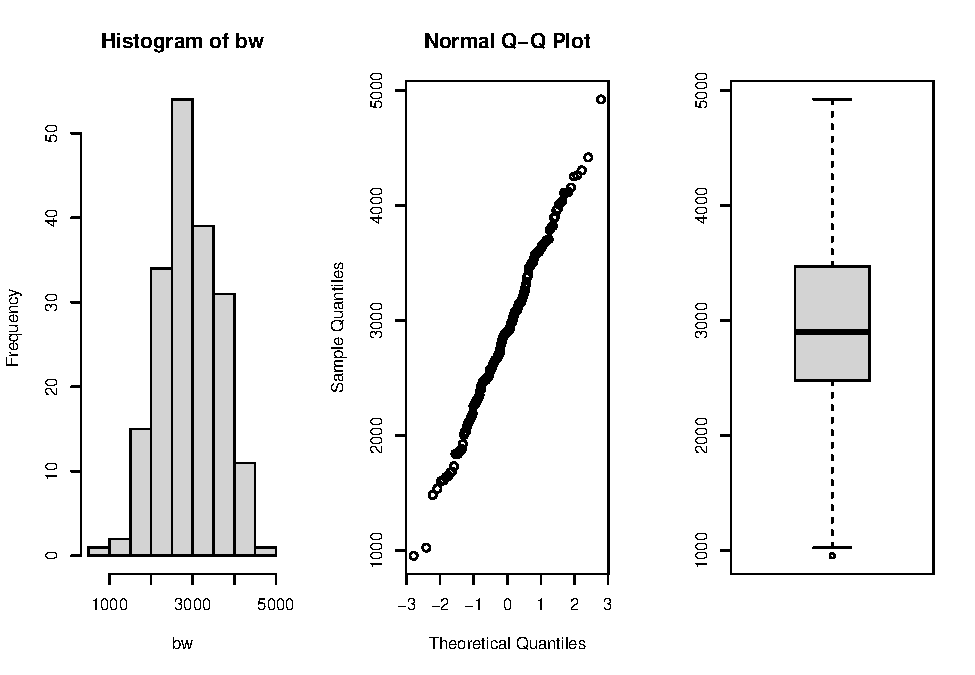
\includegraphics{Assignment-1_files/figure-latex/unnamed-chunk-1-1.pdf}

\begin{Shaded}
\begin{Highlighting}[]
\CommentTok{\# perform Shapiro{-}Wilk normality test}
\FunctionTok{round}\NormalTok{(}\FunctionTok{shapiro.test}\NormalTok{(bw)}\SpecialCharTok{$}\NormalTok{p.value, }\DecValTok{3}\NormalTok{)}
\end{Highlighting}
\end{Shaded}

\begin{verbatim}
## [1] 0.9
\end{verbatim}

The graphical methods show that the data is normal, due to the bell
shaped histogram and straight diagonal QQ-plot. The Shapiro-Wilk test
reinforces this assumption as it shows a p-value of \textgreater{} 0.05,
meaning that the \(H_0\) is not rejected and therefore the data is
normal. Furthermore, a point estimate for \(\mu\) is conducted along
side a 90\% confidence interval.

\begin{Shaded}
\begin{Highlighting}[]
\NormalTok{m }\OtherTok{=} \FunctionTok{mean}\NormalTok{(bw)}
\NormalTok{sd }\OtherTok{=} \FunctionTok{sd}\NormalTok{(bw)}
\NormalTok{n }\OtherTok{=} \FunctionTok{length}\NormalTok{(bw)}
\NormalTok{error }\OtherTok{=} \FunctionTok{qnorm}\NormalTok{(}\FloatTok{0.95}\NormalTok{)}\SpecialCharTok{*}\NormalTok{sd}\SpecialCharTok{/}\FunctionTok{sqrt}\NormalTok{(n)}
\NormalTok{ci }\OtherTok{=} \FunctionTok{c}\NormalTok{(m}\SpecialCharTok{{-}}\NormalTok{error, m}\SpecialCharTok{+}\NormalTok{error)}
\FunctionTok{paste0}\NormalTok{(}\StringTok{"mean: "}\NormalTok{, }\FunctionTok{round}\NormalTok{(m, }\DecValTok{3}\NormalTok{))}
\end{Highlighting}
\end{Shaded}

\begin{verbatim}
## [1] "mean: 2913.293"
\end{verbatim}

\begin{Shaded}
\begin{Highlighting}[]
\FunctionTok{paste0}\NormalTok{(}\StringTok{"90\% confidence interval: ("}\NormalTok{, }\FunctionTok{round}\NormalTok{(ci[}\DecValTok{1}\NormalTok{], }\DecValTok{3}\NormalTok{), }\StringTok{","}\NormalTok{, }\FunctionTok{round}\NormalTok{(ci[}\DecValTok{2}\NormalTok{], }\DecValTok{3}\NormalTok{), }\StringTok{")"}\NormalTok{)}
\end{Highlighting}
\end{Shaded}

\begin{verbatim}
## [1] "90% confidence interval: (2829.618,2996.967)"
\end{verbatim}

\textbf{b)} An expert claims that the mean birthweight is bigger than
2800, verify this claim by using a t-test. What is the outcome of the
test if you take \(\alpha\) = 0.1? And other values of \(\alpha\)?

\begin{Shaded}
\begin{Highlighting}[]
\FunctionTok{round}\NormalTok{(}\FunctionTok{t.test}\NormalTok{(bw, }\AttributeTok{mu=}\DecValTok{2800}\NormalTok{, }\AttributeTok{alternative =} \StringTok{"greater"}\NormalTok{, }\AttributeTok{conf.level =} \FloatTok{0.95}\NormalTok{)}\SpecialCharTok{$}\NormalTok{p.value, }\DecValTok{3}\NormalTok{)}
\end{Highlighting}
\end{Shaded}

\begin{verbatim}
## [1] 0.014
\end{verbatim}

A t-test is performed to verify the claim that the mean birthweight is
bigger than 2800. The t-test shows a p-value of 0.014. This means that
this claim is significant for an alpha of 0.1. The claim is significant
for all alpha's above 0.014 and insignificant for alpha's below 0.014.

\textbf{c)} In the R-output of the test from b), also a confidence
interval is given, but why is it different from the confidence interval
found in a) and why is it one-sided?

The confidence interval interval is different because the one-sample
t-test returns a 95\% confidence interval while a 90\% confidence
interval is conducted in 1b). The confidence interval is one sided
because the critical area of the weight distribution is compared to a
mean where it is greater than 2800, but not both greater and less than
2800.

\hypertarget{exercise-2}{%
\section{Exercise 2}\label{exercise-2}}

We study the power function of the two-sample t-test (see Section 1.9 of
Assignment 0). For n=m=30, mu=180, nu=175 and sd=5, generate 1000
samples x=rnorm(n,mu,sd) and y=rnorm(m,nu,sd), and record the 1000
p-values for testing H0: mu=nu. You can evaluate the power (at point
nu=175) of this t-test as fraction of p-values that are smaller than
0.05.

\textbf{a)} Set n=m=30, mu=180 and sd=5. Calculate now the power of the
t-test for every value of nu in the grid seq(175,185,by=0.25). Plot the
power as a function of nu.

\begin{Shaded}
\begin{Highlighting}[]
\NormalTok{n }\OtherTok{\textless{}{-}}\NormalTok{ m }\OtherTok{\textless{}{-}} \DecValTok{30}\NormalTok{; mu }\OtherTok{\textless{}{-}} \DecValTok{180}\NormalTok{; nu }\OtherTok{\textless{}{-}} \DecValTok{175}\NormalTok{; sd }\OtherTok{\textless{}{-}} \DecValTok{5}
\NormalTok{grid }\OtherTok{\textless{}{-}} \FunctionTok{seq}\NormalTok{(}\DecValTok{175}\NormalTok{,}\DecValTok{185}\NormalTok{, }\AttributeTok{by=}\FloatTok{0.25}\NormalTok{)}

\NormalTok{power\_function}\OtherTok{\textless{}{-}}\ControlFlowTok{function}\NormalTok{(grid,n,m,mu,sd) \{}
\NormalTok{  B }\OtherTok{\textless{}{-}} \DecValTok{1000}
\NormalTok{  p }\OtherTok{\textless{}{-}} \FunctionTok{numeric}\NormalTok{(B)}
\NormalTok{  G }\OtherTok{\textless{}{-}} \FunctionTok{length}\NormalTok{(grid)}
\NormalTok{  fractions }\OtherTok{\textless{}{-}} \FunctionTok{numeric}\NormalTok{(G)}
  \ControlFlowTok{for}\NormalTok{ (grid\_nu }\ControlFlowTok{in} \DecValTok{1}\SpecialCharTok{:}\NormalTok{G)\{}
\NormalTok{    p }\OtherTok{\textless{}{-}} \FunctionTok{numeric}\NormalTok{(B)}
    \ControlFlowTok{for}\NormalTok{ (b }\ControlFlowTok{in} \DecValTok{1}\SpecialCharTok{:}\NormalTok{B)\{}
\NormalTok{      x }\OtherTok{\textless{}{-}} \FunctionTok{rnorm}\NormalTok{(n,mu,sd)}
\NormalTok{      y }\OtherTok{\textless{}{-}} \FunctionTok{rnorm}\NormalTok{(m,grid[grid\_nu],sd)}
\NormalTok{      p[b] }\OtherTok{\textless{}{-}} \FunctionTok{t.test}\NormalTok{(x,y, }\AttributeTok{var.equal =} \ConstantTok{TRUE}\NormalTok{)[[}\DecValTok{3}\NormalTok{]]}
\NormalTok{    \}}
\NormalTok{    fractions[grid\_nu] }\OtherTok{\textless{}{-}} \FunctionTok{mean}\NormalTok{(p}\SpecialCharTok{\textless{}}\FloatTok{0.05}\NormalTok{)}
\NormalTok{  \}}
  \FunctionTok{return}\NormalTok{(fractions)}
\NormalTok{\}}

\NormalTok{fractions\_A }\OtherTok{\textless{}{-}} \FunctionTok{power\_function}\NormalTok{(grid,n,m,mu,sd)}
\end{Highlighting}
\end{Shaded}

Plots are shown further below.

\textbf{b)} Set n=m=100, mu=180 and sd=5. Repeat the preceding exercise.
Add the plot to the preceding plot.

\begin{Shaded}
\begin{Highlighting}[]
\NormalTok{n }\OtherTok{\textless{}{-}}\NormalTok{ m }\OtherTok{\textless{}{-}} \DecValTok{100}\NormalTok{; mu }\OtherTok{\textless{}{-}} \DecValTok{180}\NormalTok{; sd }\OtherTok{\textless{}{-}} \DecValTok{5}

\NormalTok{fractions\_B }\OtherTok{\textless{}{-}} \FunctionTok{power\_function}\NormalTok{(grid,n,m,mu,sd)}
\end{Highlighting}
\end{Shaded}

\textbf{c)} Set n=m=30, mu=180 and sd=15. Repeat the preceding exercise.

\begin{Shaded}
\begin{Highlighting}[]
\NormalTok{n }\OtherTok{\textless{}{-}}\NormalTok{ m }\OtherTok{\textless{}{-}} \DecValTok{30}
\NormalTok{mu }\OtherTok{\textless{}{-}} \DecValTok{180}
\NormalTok{sd }\OtherTok{\textless{}{-}} \DecValTok{15}

\NormalTok{fractions\_C }\OtherTok{\textless{}{-}} \FunctionTok{power\_function}\NormalTok{(grid,n,m,mu,sd)}
\FunctionTok{par}\NormalTok{(}\AttributeTok{mfrow=}\FunctionTok{c}\NormalTok{(}\DecValTok{1}\NormalTok{,}\DecValTok{3}\NormalTok{))}
\FunctionTok{plot}\NormalTok{(grid,fractions\_A)}
\FunctionTok{plot}\NormalTok{(grid,fractions\_B)}
\FunctionTok{plot}\NormalTok{(grid,fractions\_C)}
\end{Highlighting}
\end{Shaded}

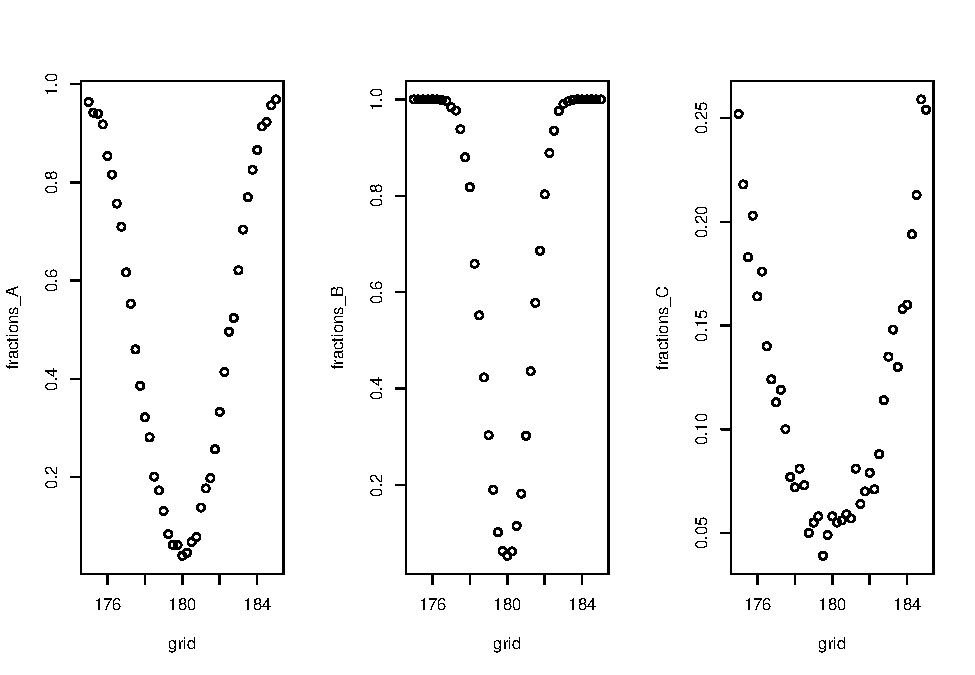
\includegraphics{Assignment-1_files/figure-latex/unnamed-chunk-6-1.pdf}

\textbf{d)} Explain your findings.

More data points seems to have an influence on the narrowness of the
plot and therefore seems to give a more precise outcome. Furthermore, a
bigger standard deviations gives a more wider distribution of fractions
as presented in the plot of C with lower values of the fractions. This
can be explained by the fact that a higher standard deviations gives a
higher uncertainty which results in a lower amount of fractions with a
p-value below 0.05.

\hypertarget{exercise-3}{%
\section{Exercise 3}\label{exercise-3}}

A telecommunication company has entered the market for mobile phones in
a new country. The company's marketing manager conducts a survey of 200
new subscribers for mobile phones. The results of the survey are in the
data set telephone.txt, which contains the first month bills
X\_1,\ldots,X\_200, in euros.

\textbf{a)} Make an appropriate plot of this data set. What marketing
advice(s) would you give to the marketing manager? Are there any
inconsistencies in the data? If so, try to fix these.

\begin{Shaded}
\begin{Highlighting}[]
\NormalTok{data}\OtherTok{\textless{}{-}}\FunctionTok{read.table}\NormalTok{(}\AttributeTok{file=}\StringTok{"data/telephone.txt"}\NormalTok{,}\AttributeTok{header=}\ConstantTok{TRUE}\NormalTok{)}

\CommentTok{\# remove zeros}
\NormalTok{data }\OtherTok{\textless{}{-}}\NormalTok{ data }\SpecialCharTok{\%\textgreater{}\%} \FunctionTok{filter}\NormalTok{(Bills }\SpecialCharTok{\textgreater{}} \DecValTok{0}\NormalTok{)}

\NormalTok{data\_tele }\OtherTok{\textless{}{-}}\NormalTok{ data}\SpecialCharTok{$}\NormalTok{Bills}
\FunctionTok{par}\NormalTok{(}\AttributeTok{mfrow=}\FunctionTok{c}\NormalTok{(}\DecValTok{1}\NormalTok{,}\DecValTok{3}\NormalTok{))}
\FunctionTok{hist}\NormalTok{(data\_tele)}
\FunctionTok{qqnorm}\NormalTok{(data\_tele)}
\FunctionTok{boxplot}\NormalTok{(data\_tele)}
\end{Highlighting}
\end{Shaded}

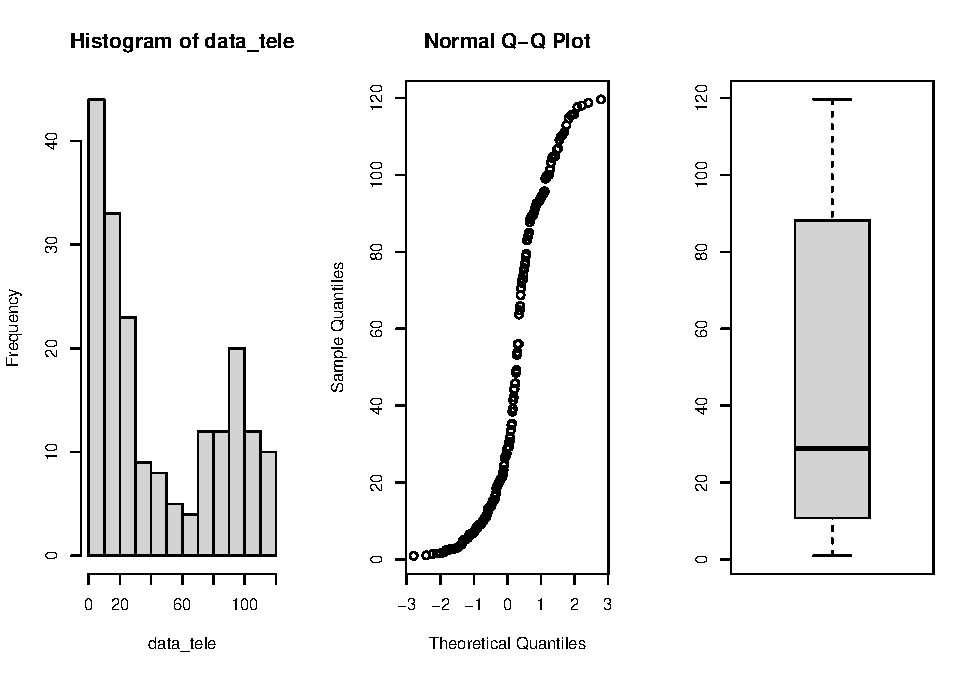
\includegraphics{Assignment-1_files/figure-latex/unnamed-chunk-7-1.pdf}

From the survey it seems that there are two distinct peaks,therefore it
would be good to run two separate marketing campaigns: a ``premium''
service campaign for customers who are willing to spend more and a
campaign aimed at savers, usually people who use pre-paid services, -
establishing a separate ``cheaper'' brand would be a good strategy here.

The survey data also encompassed people who did not have any spendings
on the phone bills, therefore they were removed from the analysis.

\textbf{b)} By using a bootstrap test with the test statistic T =
median(\(X_1,....,X_200\)), test whether the data telephone.txt stems
from the exponential distribution Exp(\(\lambda\)) with some lambda from
{[}0.01, 0.1{]}.

\begin{Shaded}
\begin{Highlighting}[]
\NormalTok{lambda }\OtherTok{\textless{}{-}} \FunctionTok{seq}\NormalTok{(}\FloatTok{0.01}\NormalTok{, }\FloatTok{0.1}\NormalTok{, }\FloatTok{0.0005}\NormalTok{)}
\NormalTok{pvalues }\OtherTok{\textless{}{-}} \FunctionTok{c}\NormalTok{()}
\NormalTok{t }\OtherTok{\textless{}{-}} \FunctionTok{median}\NormalTok{(data\_tele)}
\ControlFlowTok{for}\NormalTok{ (x }\ControlFlowTok{in}\NormalTok{ lambda)\{}
\NormalTok{  B }\OtherTok{\textless{}{-}} \DecValTok{1000}
\NormalTok{  tstar }\OtherTok{\textless{}{-}} \FunctionTok{numeric}\NormalTok{(B)}
\NormalTok{  n }\OtherTok{\textless{}{-}} \FunctionTok{length}\NormalTok{(data\_tele)}
  
  \ControlFlowTok{for}\NormalTok{ (i }\ControlFlowTok{in} \DecValTok{1}\SpecialCharTok{:}\NormalTok{B)\{}
\NormalTok{    xstar }\OtherTok{\textless{}{-}} \FunctionTok{rexp}\NormalTok{(n,x)}
\NormalTok{    tstar[i] }\OtherTok{\textless{}{-}} \FunctionTok{median}\NormalTok{(xstar)}
\NormalTok{  \}}
\NormalTok{  pl}\OtherTok{\textless{}{-}}\FunctionTok{sum}\NormalTok{(tstar}\SpecialCharTok{\textless{}}\NormalTok{t)}\SpecialCharTok{/}\NormalTok{B}
\NormalTok{  pr}\OtherTok{\textless{}{-}}\FunctionTok{sum}\NormalTok{(tstar}\SpecialCharTok{\textgreater{}}\NormalTok{t)}\SpecialCharTok{/}\NormalTok{B}
\NormalTok{  p}\OtherTok{\textless{}{-}}\DecValTok{2}\SpecialCharTok{*}\FunctionTok{min}\NormalTok{(pl,pr)}
\NormalTok{  pl;pr;p}
\NormalTok{  pvalues }\OtherTok{\textless{}{-}} \FunctionTok{c}\NormalTok{(pvalues,p)}
\NormalTok{\}}
\FunctionTok{plot}\NormalTok{(lambda, pvalues)}
\end{Highlighting}
\end{Shaded}

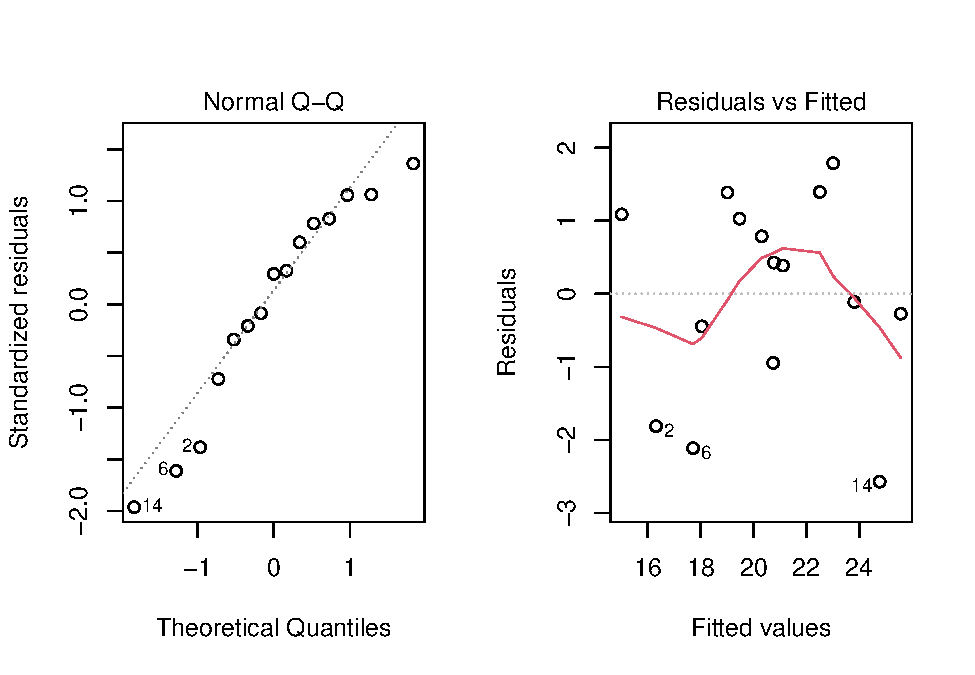
\includegraphics{Assignment-1_files/figure-latex/unnamed-chunk-8-1.pdf}

\begin{Shaded}
\begin{Highlighting}[]
\NormalTok{best\_p }\OtherTok{\textless{}{-}} \FunctionTok{which}\NormalTok{(pvalues }\SpecialCharTok{\textgreater{}} \FloatTok{0.05}\NormalTok{)}
\NormalTok{lambda[best\_p]}
\end{Highlighting}
\end{Shaded}

\begin{verbatim}
##  [1] 0.0195 0.0200 0.0205 0.0210 0.0215 0.0220 0.0225 0.0230 0.0235 0.0240
## [11] 0.0245 0.0250 0.0255 0.0260 0.0265 0.0270 0.0275 0.0280 0.0285 0.0290
## [21] 0.0295
\end{verbatim}

The figure above shows the p-values for different lambda values. There
can be concluded that the data stems from a exponential distribution for
the lambda values 0.02 to 0.029.

\textbf{c)} Construct a 95\% bootstrap confidence interval for the
population median of the sample.

\begin{Shaded}
\begin{Highlighting}[]
\NormalTok{B }\OtherTok{\textless{}{-}} \DecValTok{1000}
\NormalTok{T1 }\OtherTok{\textless{}{-}} \FunctionTok{median}\NormalTok{(data\_tele)}
\NormalTok{Tstar }\OtherTok{\textless{}{-}} \FunctionTok{numeric}\NormalTok{(B)}
\ControlFlowTok{for}\NormalTok{ (i }\ControlFlowTok{in} \DecValTok{1}\SpecialCharTok{:}\NormalTok{B)\{}
\NormalTok{  Xstar }\OtherTok{\textless{}{-}} \FunctionTok{sample}\NormalTok{(data\_tele,}\AttributeTok{replace=}\ConstantTok{TRUE}\NormalTok{)}
\NormalTok{  Tstar[i] }\OtherTok{\textless{}{-}} \FunctionTok{median}\NormalTok{(Xstar)}
\NormalTok{\}}
\NormalTok{Tstar25 }\OtherTok{\textless{}{-}} \FunctionTok{quantile}\NormalTok{(Tstar,}\FloatTok{0.025}\NormalTok{)}
\NormalTok{Tstar975 }\OtherTok{\textless{}{-}} \FunctionTok{quantile}\NormalTok{(Tstar, }\FloatTok{0.975}\NormalTok{)}

\FunctionTok{paste0}\NormalTok{(}\StringTok{"Data median: "}\NormalTok{, }\FunctionTok{round}\NormalTok{(T1, }\DecValTok{3}\NormalTok{))}
\end{Highlighting}
\end{Shaded}

\begin{verbatim}
## [1] "Data median: 28.905"
\end{verbatim}

\begin{Shaded}
\begin{Highlighting}[]
\FunctionTok{paste0}\NormalTok{(}\StringTok{"95\% confidence interval: ("}\NormalTok{, }\FunctionTok{round}\NormalTok{(}\DecValTok{2}\SpecialCharTok{*}\NormalTok{T1}\SpecialCharTok{{-}}\NormalTok{Tstar975, }\DecValTok{3}\NormalTok{), }
       \StringTok{","}\NormalTok{, }\FunctionTok{round}\NormalTok{(}\DecValTok{2}\SpecialCharTok{*}\NormalTok{T1}\SpecialCharTok{{-}}\NormalTok{Tstar25, }\DecValTok{3}\NormalTok{), }\StringTok{")"}\NormalTok{)}
\end{Highlighting}
\end{Shaded}

\begin{verbatim}
## [1] "95% confidence interval: (17.093,36.64)"
\end{verbatim}

The 95\% bootstrap confidence interval of the median can be observed
above. The confidence interval of the bootstrap method changes each time
it is executed because of the random nature of the method.

\textbf{d)} Assuming \(X_1,....,X_n ~ Exp(\lambda)\) and using the
central limit theorem for the sample mean, estimate lambda and construct
again a 95\% confidence interval for the population median. Comment on
your findings.

The variable opt\_Lambda is the lambda value for which the p-value was
the highest. The CLT allows us to compute a normal confidence intervals
to data that are not themselves normally distributed and therefore can
be used to the exponentially distributed data. To do this for the
median, a theoretical median needs to be computed, which can be found in
the following way: \(\frac{ln(2)}{\lambda}\). The confidence interval of
the median can be computed with the found theoretical median.

\begin{Shaded}
\begin{Highlighting}[]
\NormalTok{max\_index }\OtherTok{\textless{}{-}} \FunctionTok{which.max}\NormalTok{(pvalues)}

\NormalTok{opt\_Lambda }\OtherTok{\textless{}{-}}\NormalTok{ lambda[max\_index]}

\FunctionTok{paste0}\NormalTok{(}\StringTok{"Optimal lambda value found: "}\NormalTok{, }\FunctionTok{round}\NormalTok{(opt\_Lambda, }\DecValTok{3}\NormalTok{))}
\end{Highlighting}
\end{Shaded}

\begin{verbatim}
## [1] "Optimal lambda value found: 0.024"
\end{verbatim}

\begin{Shaded}
\begin{Highlighting}[]
\CommentTok{\# simulate exponential distribution and calculate the ci}
\NormalTok{medians }\OtherTok{\textless{}{-}} \FunctionTok{c}\NormalTok{()}
\NormalTok{B }\OtherTok{\textless{}{-}} \DecValTok{1000}
\NormalTok{n }\OtherTok{\textless{}{-}} \FunctionTok{length}\NormalTok{(data\_tele)}

\ControlFlowTok{for}\NormalTok{ (i }\ControlFlowTok{in} \DecValTok{1}\SpecialCharTok{:}\NormalTok{B)\{}
\NormalTok{  medians }\OtherTok{\textless{}{-}} \FunctionTok{c}\NormalTok{(medians, }\FunctionTok{median}\NormalTok{(}\FunctionTok{rexp}\NormalTok{(n,opt\_Lambda)))}
\NormalTok{\}}

\NormalTok{sd }\OtherTok{=} \FunctionTok{sd}\NormalTok{(medians)}
\NormalTok{m }\OtherTok{=} \FunctionTok{mean}\NormalTok{(medians)}
\NormalTok{error }\OtherTok{=} \FunctionTok{qnorm}\NormalTok{(}\FloatTok{0.975}\NormalTok{)}\SpecialCharTok{*}\NormalTok{sd}\SpecialCharTok{/}\FunctionTok{sqrt}\NormalTok{(B)}
\NormalTok{ci }\OtherTok{=} \FunctionTok{c}\NormalTok{(m}\SpecialCharTok{{-}}\NormalTok{error, m}\SpecialCharTok{+}\NormalTok{error)}
\FunctionTok{paste0}\NormalTok{(}\StringTok{"Median estimate: "}\NormalTok{, }\FunctionTok{round}\NormalTok{(m, }\DecValTok{3}\NormalTok{))}
\end{Highlighting}
\end{Shaded}

\begin{verbatim}
## [1] "Median estimate: 29.009"
\end{verbatim}

\begin{Shaded}
\begin{Highlighting}[]
\FunctionTok{paste0}\NormalTok{(}\StringTok{"95\% confidence interval: ("}\NormalTok{, }\FunctionTok{round}\NormalTok{(ci[}\DecValTok{1}\NormalTok{], }\DecValTok{3}\NormalTok{), }\StringTok{","}\NormalTok{, }\FunctionTok{round}\NormalTok{(ci[}\DecValTok{2}\NormalTok{], }\DecValTok{3}\NormalTok{), }\StringTok{")"}\NormalTok{)}
\end{Highlighting}
\end{Shaded}

\begin{verbatim}
## [1] "95% confidence interval: (28.817,29.201)"
\end{verbatim}

Optimal \(\lambda\) was selected from the experiment in b) that resulted
in the highest p-value. The results show a 95\% confidence interval that
is more narrow than the one found via bootstrapping. This is attributed
to the stochastic nature of the bootstrap and the fact that bootstrap
used real data clearly deviated from perfect exponential distribution.

\textbf{e)} Using an appropriate test, test the null hypothesis that the
median bill is bigger or equal to 40 euro against the alternative that
the median bill is smaller than 40 euro. Next, design and perform a test
to check whether the fraction of the bills less than 10 euro is less
than 25\%.

\begin{Shaded}
\begin{Highlighting}[]
\NormalTok{bill\_smal40 }\OtherTok{\textless{}{-}} \FunctionTok{sum}\NormalTok{(data\_tele}\SpecialCharTok{\textless{}}\DecValTok{40}\NormalTok{)}

\FunctionTok{binom.test}\NormalTok{(bill\_smal40, }\FunctionTok{length}\NormalTok{(data\_tele))}
\end{Highlighting}
\end{Shaded}

\begin{verbatim}
## 
##  Exact binomial test
## 
## data:  bill_smal40 and length(data_tele)
## number of successes = 109, number of trials = 192, p-value = 0.07
## alternative hypothesis: true probability of success is not equal to 0.5
## 95 percent confidence interval:
##  0.494 0.639
## sample estimates:
## probability of success 
##                  0.568
\end{verbatim}

\begin{Shaded}
\begin{Highlighting}[]
\NormalTok{bill\_less10 }\OtherTok{\textless{}{-}} \FunctionTok{sum}\NormalTok{(data\_tele }\SpecialCharTok{\textless{}} \DecValTok{10}\NormalTok{)}
\NormalTok{bill\_less10}\SpecialCharTok{/}\FunctionTok{length}\NormalTok{(data\_tele)}
\end{Highlighting}
\end{Shaded}

\begin{verbatim}
## [1] 0.229
\end{verbatim}

In the above cell one can observe that a binomial test is used with as
x-value the data of the telephone company where the bills where lower
than 40 euro. The null hypothesis of this test states that that the
median bill is bigger or equal to 40 euro while the alternative
hypothesis states that the the median bill is smaller than 40 euro.
After conducted this test a p-value of 0.07 is found, which means that
the Null hypothesis can not be rejected as it is higher than the
standard alpha of 0.05. This also means that the alternative hypothesis
can not be accepted. Furthermore a test is conducted to see whether the
fraction of the bills less than 10 euro is less than 25\%. In the above
cell can be seen that the fraction is equal to 0.229 which is smaller
than 0.25 and therefore we can state that the fraction is less than
25\%.

\hypertarget{exercise-4}{%
\section{Exercise 4}\label{exercise-4}}

To study the effect of energy drink a sample of 24 high school pupils
were randomized to drinking either a softdrink or an energy drink after
running for 60 meters. After half an hour they were asked to run again.
For both sprints they were asked to sprint as fast they could, and the
sprinting time was measured. The data is given in the file run.txt.
{[}Courtesy class 5E, Stedelijk Gymnasium Leiden, 2010.{]}

\textbf{a)} Disregarding the type of drink, test whether the run times
before drink and after are correlated.

\begin{Shaded}
\begin{Highlighting}[]
\NormalTok{data }\OtherTok{\textless{}{-}} \FunctionTok{read.table}\NormalTok{(}\AttributeTok{file=}\StringTok{"data/run.txt"}\NormalTok{,}\AttributeTok{header=}\ConstantTok{TRUE}\NormalTok{)}
\FunctionTok{cor.test}\NormalTok{(data}\SpecialCharTok{$}\NormalTok{before, data}\SpecialCharTok{$}\NormalTok{after)}\SpecialCharTok{$}\NormalTok{p.value}
\end{Highlighting}
\end{Shaded}

\begin{verbatim}
## [1] 0.00078
\end{verbatim}

\begin{Shaded}
\begin{Highlighting}[]
\DocumentationTok{\#\# disgnostics}
\FunctionTok{par}\NormalTok{(}\AttributeTok{mfrow=}\FunctionTok{c}\NormalTok{(}\DecValTok{1}\NormalTok{,}\DecValTok{2}\NormalTok{)); }\FunctionTok{qqnorm}\NormalTok{(data}\SpecialCharTok{$}\NormalTok{before); }\FunctionTok{qqnorm}\NormalTok{(data}\SpecialCharTok{$}\NormalTok{after)}
\end{Highlighting}
\end{Shaded}

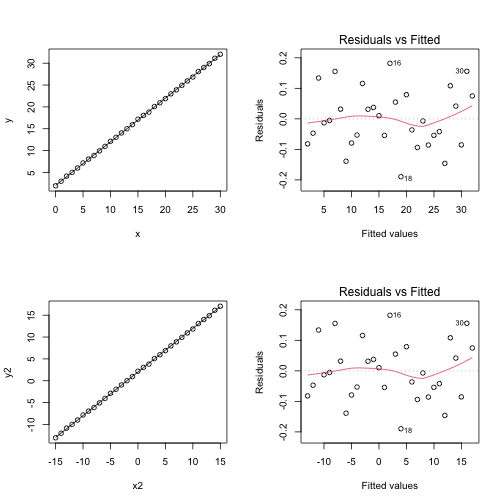
\includegraphics{Assignment-1_files/figure-latex/unnamed-chunk-12-1.pdf}

To test whether the data is correlated we run a Pearson correlation
test. From the resulting p-value above we can conclude that there is
significant correlation between the running times before drink and after
drink. Assumption of normality needed for the performed test was
confirmed by a qqnorm plot.

\textbf{b)} Test separately, for both the softdrink and the energy drink
conditions, whether there is a difference in speed in the two running
tasks.

\begin{Shaded}
\begin{Highlighting}[]
\CommentTok{\# calculate differences}
\NormalTok{data }\OtherTok{\textless{}{-}}\NormalTok{ data }\SpecialCharTok{\%\textgreater{}\%} 
  \FunctionTok{mutate}\NormalTok{(}\AttributeTok{diff =}\NormalTok{ before }\SpecialCharTok{{-}}\NormalTok{ after)}
\CommentTok{\# filter for lemo and perdorm paired t{-}test}
\NormalTok{lemo }\OtherTok{\textless{}{-}}\NormalTok{ data }\SpecialCharTok{\%\textgreater{}\%} 
  \FunctionTok{filter}\NormalTok{(drink }\SpecialCharTok{==} \StringTok{"lemo"}\NormalTok{)}
\FunctionTok{paste0}\NormalTok{(}\StringTok{"p{-}value for soft drink: "}\NormalTok{, }
       \FunctionTok{round}\NormalTok{(}\FunctionTok{t.test}\NormalTok{(lemo}\SpecialCharTok{$}\NormalTok{before, lemo}\SpecialCharTok{$}\NormalTok{after, }\AttributeTok{paired =} \ConstantTok{TRUE}\NormalTok{)}\SpecialCharTok{$}\NormalTok{p.value, }\DecValTok{3}\NormalTok{))}
\end{Highlighting}
\end{Shaded}

\begin{verbatim}
## [1] "p-value for soft drink: 0.437"
\end{verbatim}

\begin{Shaded}
\begin{Highlighting}[]
\CommentTok{\# filter for energy and perform paired t{-}test}
\NormalTok{energy }\OtherTok{\textless{}{-}}\NormalTok{ data }\SpecialCharTok{\%\textgreater{}\%} 
  \FunctionTok{filter}\NormalTok{(drink }\SpecialCharTok{==} \StringTok{"energy"}\NormalTok{)}
\FunctionTok{paste0}\NormalTok{(}\StringTok{"p{-}value for energy drink: "}\NormalTok{, }
       \FunctionTok{round}\NormalTok{(}\FunctionTok{t.test}\NormalTok{(energy}\SpecialCharTok{$}\NormalTok{before, energy}\SpecialCharTok{$}\NormalTok{after, }\AttributeTok{paired =} \ConstantTok{TRUE}\NormalTok{)}\SpecialCharTok{$}\NormalTok{p.value, }\DecValTok{3}\NormalTok{))}
\end{Highlighting}
\end{Shaded}

\begin{verbatim}
## [1] "p-value for energy drink: 0.126"
\end{verbatim}

Paired t-test was selected for this task as the experimental data was
collected for the same individual after and before drink. For both
energy and soft-drink groups there does not seem to be a significant
difference in means of the running times as the p-values are \textless{}
0.05.

\textbf{c)} For each pupil compute the time difference between the two
running tasks. Test whether these time differences are effected by the
type of drink.

\begin{Shaded}
\begin{Highlighting}[]
\CommentTok{\# perform t{-}test}
\FunctionTok{t.test}\NormalTok{(lemo}\SpecialCharTok{$}\NormalTok{diff, energy}\SpecialCharTok{$}\NormalTok{diff)}\SpecialCharTok{$}\NormalTok{p.value}
\end{Highlighting}
\end{Shaded}

\begin{verbatim}
## [1] 0.159
\end{verbatim}

The p-value is \textgreater{} 0.05, therefore the means of the two
populations are not significantly different.

\textbf{d)} Can you think of a plausible objection to the design of the
experiment in b) if the main aim was to test whether drinking the energy
drink speeds up the running? Is there a similar objection to the design
of the experiment in c)? Comment on all your findings in this exercise.

In both experiments the participants were asked to run on the same day.
This could strongly influence the outcomes in data. Therefore, the setup
was certainly not ideal to check the influence of both drinks. Same
objection does not hold for the experiment in c) since both of the
groups were independent and underwent same experimental conditions.

\hypertarget{exercise-5}{%
\section{Exercise 5}\label{exercise-5}}

\textbf{a)} Test whether the distributions of the chicken weights for
meatmeal and sunflower groups are different by performing three tests:
the two samples t-test (argue whether the data are paired or not), the
Mann-Whitney test and the Kolmogorov-Smirnov test. Comment on your
findings.

\begin{Shaded}
\begin{Highlighting}[]
\CommentTok{\# filter for meatmeal}
\NormalTok{meatmeal }\OtherTok{\textless{}{-}}\NormalTok{ chickwts }\SpecialCharTok{\%\textgreater{}\%} 
  \FunctionTok{filter}\NormalTok{(feed }\SpecialCharTok{==} \StringTok{"meatmeal"}\NormalTok{) }\SpecialCharTok{\%\textgreater{}\%} 
  \FunctionTok{select}\NormalTok{(weight)}
\CommentTok{\# filter for sunflower}
\NormalTok{sunflower }\OtherTok{\textless{}{-}}\NormalTok{ chickwts }\SpecialCharTok{\%\textgreater{}\%} 
  \FunctionTok{filter}\NormalTok{(feed }\SpecialCharTok{==} \StringTok{"sunflower"}\NormalTok{) }\SpecialCharTok{\%\textgreater{}\%} 
  \FunctionTok{select}\NormalTok{(weight)}
\CommentTok{\# check for data normality}
\FunctionTok{par}\NormalTok{(}\AttributeTok{mfrow=}\FunctionTok{c}\NormalTok{(}\DecValTok{1}\NormalTok{,}\DecValTok{2}\NormalTok{))}
\FunctionTok{qqnorm}\NormalTok{(meatmeal}\SpecialCharTok{$}\NormalTok{weight)}
\FunctionTok{qqnorm}\NormalTok{(sunflower}\SpecialCharTok{$}\NormalTok{weight)}
\end{Highlighting}
\end{Shaded}

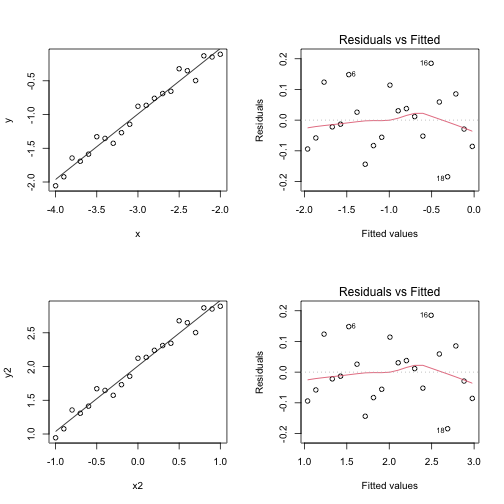
\includegraphics{Assignment-1_files/figure-latex/unnamed-chunk-15-1.pdf}

\begin{Shaded}
\begin{Highlighting}[]
\CommentTok{\# perform t{-}test, the data is not paired}
\FunctionTok{paste0}\NormalTok{(}\StringTok{"t{-}test p{-}value: "}\NormalTok{, }
       \FunctionTok{round}\NormalTok{(}\FunctionTok{t.test}\NormalTok{(meatmeal, sunflower)}\SpecialCharTok{$}\NormalTok{p.value, }\DecValTok{3}\NormalTok{))}
\end{Highlighting}
\end{Shaded}

\begin{verbatim}
## [1] "t-test p-value: 0.044"
\end{verbatim}

\begin{Shaded}
\begin{Highlighting}[]
\CommentTok{\# Mann{-}Whitney test}
\FunctionTok{paste0}\NormalTok{(}\StringTok{"Mann{-}Whitney test p{-}value: "}\NormalTok{, }
       \FunctionTok{round}\NormalTok{(}\FunctionTok{wilcox.test}\NormalTok{(meatmeal}\SpecialCharTok{$}\NormalTok{weight, sunflower}\SpecialCharTok{$}\NormalTok{weight)}\SpecialCharTok{$}\NormalTok{p.value, }\DecValTok{3}\NormalTok{))}
\end{Highlighting}
\end{Shaded}

\begin{verbatim}
## [1] "Mann-Whitney test p-value: 0.069"
\end{verbatim}

\begin{Shaded}
\begin{Highlighting}[]
\CommentTok{\# Kolmogorov{-}Smirnov test}
\FunctionTok{paste0}\NormalTok{(}\StringTok{"Kolmogorov{-}Smirnov test: "}\NormalTok{, }
       \FunctionTok{round}\NormalTok{(}\FunctionTok{ks.test}\NormalTok{(meatmeal}\SpecialCharTok{$}\NormalTok{weight, sunflower}\SpecialCharTok{$}\NormalTok{weight)}\SpecialCharTok{$}\NormalTok{p.value, }\DecValTok{3}\NormalTok{))}
\end{Highlighting}
\end{Shaded}

\begin{verbatim}
## [1] "Kolmogorov-Smirnov test: 0.108"
\end{verbatim}

Data in chickwts is not paired as the ``treatment'' of different feed
was applied to different newly-hatched chicks, therefore the data is
independent. From t-test we can see that the p-values \textless0.05,
this would conclude that the means between the two groups are
significantly different. From Mann-Whitney test we can see that p-value
is \textgreater0.05, therefore we cannot conclude that the medians of
the two datasets are different. From Kolgomorov-Smirnov test we can see
that p-value is \textgreater0.05, therefore we cannot conclude that the
means are different. From qqnorm plots we can observe that the
``sunflower'' feed data is not normal, therefore t-test here is
inappropriate.

\textbf{b)}Conduct a one-way ANOVA to determine whether the type of feed
supplement has an effect on the weight of the chicks. Give the estimated
chick weights for each of the six feed supplements. What is the best
feed supplement?

\begin{Shaded}
\begin{Highlighting}[]
\NormalTok{chickaov }\OtherTok{\textless{}{-}} \FunctionTok{lm}\NormalTok{(weight}\SpecialCharTok{\textasciitilde{}}\NormalTok{feed, }\AttributeTok{data =}\NormalTok{ chickwts)}
\CommentTok{\# performing one{-}way ANOVA}
\FunctionTok{anova}\NormalTok{(chickaov)}
\end{Highlighting}
\end{Shaded}

\begin{verbatim}
## Analysis of Variance Table
## 
## Response: weight
##           Df Sum Sq Mean Sq F value  Pr(>F)    
## feed       5 231129   46226    15.4 5.9e-10 ***
## Residuals 65 195556    3009                    
## ---
## Signif. codes:  0 '***' 0.001 '**' 0.01 '*' 0.05 '.' 0.1 ' ' 1
\end{verbatim}

From the results of one-way ANOVA we can see that the p-values is
\textless{} 0.05, therefore we can conclude that at least one of the
means between different feed varieties are significantly different from
the rest.

\begin{Shaded}
\begin{Highlighting}[]
\CommentTok{\#extracting more information}
\NormalTok{table }\OtherTok{\textless{}{-}} \FunctionTok{data.frame}\NormalTok{(}\FunctionTok{summary}\NormalTok{(chickaov)}\SpecialCharTok{$}\NormalTok{coefficients) }
\NormalTok{table }\SpecialCharTok{\%\textgreater{}\%} 
  \FunctionTok{rename}\NormalTok{(}\StringTok{"p{-}value"} \OtherTok{=} \StringTok{\textasciigrave{}}\AttributeTok{Pr...t..}\StringTok{\textasciigrave{}}\NormalTok{) }\SpecialCharTok{\%\textgreater{}\%} 
  \FunctionTok{add\_rownames}\NormalTok{(}\StringTok{"Type"}\NormalTok{) }\SpecialCharTok{\%\textgreater{}\%} 
  \FunctionTok{mutate}\NormalTok{(}\AttributeTok{Type =} \FunctionTok{case\_when}\NormalTok{(}
\NormalTok{    Type }\SpecialCharTok{==} \StringTok{"(Intercept)"} \SpecialCharTok{\textasciitilde{}} \StringTok{"feedcasein"}\NormalTok{,}
    \ConstantTok{TRUE} \SpecialCharTok{\textasciitilde{}}\NormalTok{ Type}
\NormalTok{  ), }\AttributeTok{Estimate =} \FunctionTok{case\_when}\NormalTok{(}
\NormalTok{    Type }\SpecialCharTok{!=} \StringTok{"feedcasein"} \SpecialCharTok{\textasciitilde{}} \FunctionTok{as.numeric}\NormalTok{(table}\SpecialCharTok{$}\NormalTok{Estimate[}\DecValTok{1}\NormalTok{]) }\SpecialCharTok{+}\NormalTok{ Estimate,}
    \ConstantTok{TRUE} \SpecialCharTok{\textasciitilde{}}\NormalTok{ Estimate}
\NormalTok{  )) }\SpecialCharTok{\%\textgreater{}\%}  \FunctionTok{mutate\_if}\NormalTok{(is.numeric, }\FunctionTok{funs}\NormalTok{(}\FunctionTok{as.character}\NormalTok{(}\FunctionTok{signif}\NormalTok{(., }\DecValTok{3}\NormalTok{)))) }\SpecialCharTok{\%\textgreater{}\%}
\NormalTok{    knitr}\SpecialCharTok{::}\FunctionTok{kable}\NormalTok{(.)}
\end{Highlighting}
\end{Shaded}

\begin{longtable}[]{@{}lllll@{}}
\toprule
Type & Estimate & Std..Error & t.value & p-value\tabularnewline
\midrule
\endhead
feedcasein & 324 & 15.8 & 20.4 & 5.33e-30\tabularnewline
feedhorsebean & 160 & 23.5 & -6.96 & 2.07e-09\tabularnewline
feedlinseed & 219 & 22.4 & -4.68 & 1.49e-05\tabularnewline
feedmeatmeal & 277 & 22.9 & -2.04 & 0.0456\tabularnewline
feedsoybean & 246 & 21.6 & -3.58 & 0.000665\tabularnewline
feedsunflower & 329 & 22.4 & 0.238 & 0.812\tabularnewline
\bottomrule
\end{longtable}

From summary statistics it seems that ``sunflower'' feed is the feed
resulting in the highest weight, however by looking at the p-values we
can see that it is not significantly different from ``casein'' feed
variety, therefore we cannot conclude which one of these two is the
best.

\textbf{c)}Check the ANOVA model assumptions by using relevant
diagnostic tools.

\begin{Shaded}
\begin{Highlighting}[]
\CommentTok{\# check for normality}
\FunctionTok{qqnorm}\NormalTok{(chickaov}\SpecialCharTok{$}\NormalTok{residuals)}
\end{Highlighting}
\end{Shaded}

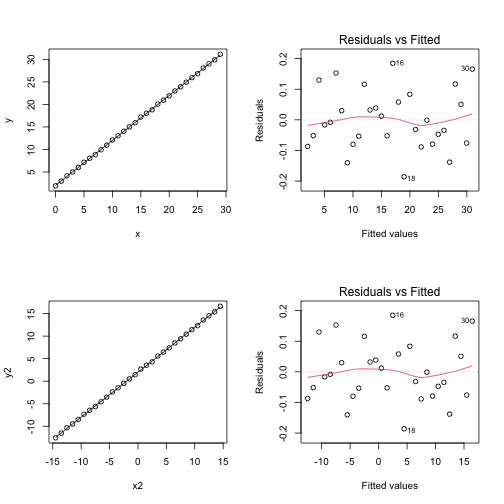
\includegraphics{Assignment-1_files/figure-latex/unnamed-chunk-18-1.pdf}

From qqplot the assumption of normality holds.

\textbf{d)} Does the Kruskal-Wallis test arrive at the same conclusion
about the effect of feed supplement as the test in b)? Explain possible
differences between conclusions of the Kruskal-Wallis and ANOVA tests.

\begin{Shaded}
\begin{Highlighting}[]
\FunctionTok{kruskal.test}\NormalTok{(weight}\SpecialCharTok{\textasciitilde{}}\NormalTok{feed, }\AttributeTok{data =}\NormalTok{ chickwts)}\SpecialCharTok{$}\NormalTok{p.value}
\end{Highlighting}
\end{Shaded}

\begin{verbatim}
## [1] 5.11e-07
\end{verbatim}

With Kruskal-Wallis test we arrive to the same conclusion as with ANOVA.
This is an expected outcome as ANOVA works with normal data (assumption
verified in c) and Kruskal-Wallis test works with any type of data.

\end{document}
